\section{РАЗРАБОТАННОЕ РЕШЕНИЕ}

\subsection{Подход к решению данной задачи}

При разработке решения для облегчения работы врачей и медицинского персонала в области справочной информации, был выбран системный подход, включающий следующие этапы:
\begin{itemize}

 \item исследование и анализ потребностей. В начале процесса были проведены исследования и анализ потребностей врачей и медицинского персонала. Перед началом всей работы мы встречались с медицинском работником, который рассказал о своих возражениях и о том, какой результат хотел бы получить:
 \begin{itemize}
     \item в настоящий момент после каждого вызова врач скорой помощи должен заполнять документ, который назвается <<Карта вызова>>. составлена в соответствии с формой №110/у «Карта вызова скорой медицинской помощи», утвержденной  приказом Минздравсоцразвития России от 02.12.2009г. №942 «Об утверждении статистического инструментария станции (отделения), больницы скорой медицинской помощи», с учетом требований приказов по Станции и обработки данных в КАСУ. «Карта вызова» является юридическим медицинским документом, единым для всех бригад Станции скорой медицинской помощи по выполнению вызовов поступающих на Станцию. «Карта вызова» заполняется на каждый вызов аккуратным и разборчивым почерком. В случае повторного ее заполнения к ней прилагается объяснение с указанием его причин.
     В связи с этим врачу стоит предоставить возможность исправить данные, внесенный в карту до того, как она будет распечатана. В электронном варианте это сделать проще всего;
     \item в карту многие из пунктов вносятся вручную. Задача состоит в том, чтобы предоставить врачу иметь возможность выбрать набор действий по оказанию помощи, который связан с определнным кодом МКБ, который автоматически будет заноситься в карту вызова в раздел оказанной помощи. Если врач захочет, то он сможет исправить занесенную информацию или дополнить ее новой.
 \end{itemize};

 \item определение функциональных требований. На основе полученных данных были определены основные функциональные требования к разрабатываемому решению. Это включало функции поиска, навигации, визуализации алгоритмов и доступа к актуальной информации, предоставленной врачом;

 \item проектирование интерфейса и архитектуры. Был разработан удобный и интуитивно понятный интерфейс, который позволяет пользователям легко находить и получать необходимую информацию, после чего можно ее сохранить и внести в карту вызова. Была такая спроектирована архитектура решения, которая учитывает интеграцию с другими системами;

 \item разработка и тестирование. На основе определенных требований и проектирования была проведена разработка интерфейса. Были созданы функциональность поиска, визуализации алгоритмов и доступа к справочной информации. Затем проводились тестирования для проверки работоспособности, удобства использования и соответствия требованиям.

\end{itemize}

На рисунке~\ref{fig:fig09} приведена карта вызовов, которая используется нашим консультирующим врачом. Выбранные пункты окзанной помощь заносятся в раздел карты <<Оказанная помощь и ее эффект>>.

     \begin{figure}
        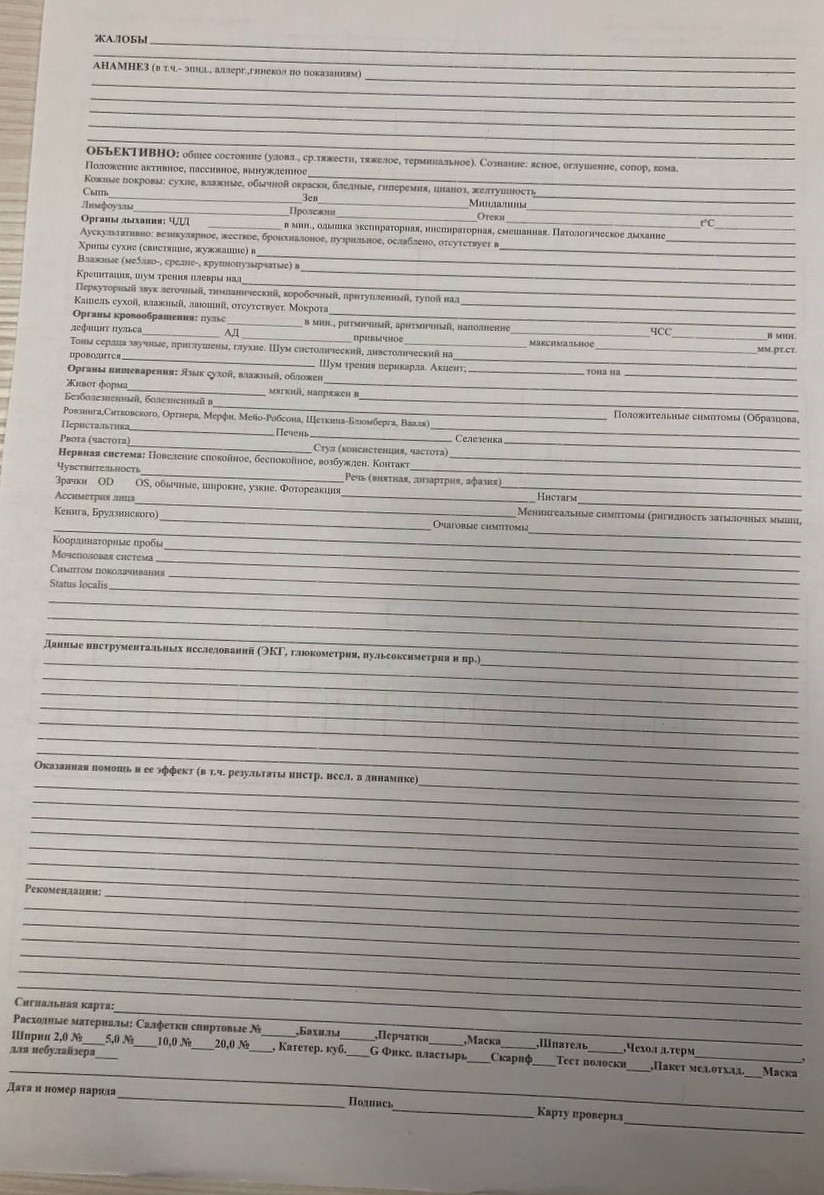
\includegraphics[scale=0.6]{styles/diploma/inc/card_medics.jpg}
        \caption{Карта вызова}
        \label{fig:fig09}
    \end{figure}




В результате системного подхода к разработке решения для справочной информации было достигнуто создание инновационного медицинского приложения, которое с учетом потребностей и запросов врачей предоставляет удобный и эффективный функционал для поддержки медицинской практики.

\subsection{Стек используемых технологий}
\subsubsection{Работа с данными}

В веб-приложениях данные могут храниться в различных местах в зависимости от их типа, объема и требований приложения. Вот некоторые распространенные места хранения данных в веб-приложениях:
\begin{itemize}
    \item база данных. Одним из основных и наиболее распространенных мест хранения данных в веб-приложениях является база данных. Базы данных могут быть реляционными (например, MySQL, PostgreSQL) или нереляционными (например, MongoDB, Cassandra) в зависимости от типа данных и требований приложения. Базы данных обеспечивают постоянное хранение данных и предоставляют возможности поиска, фильтрации и изменения данных;
    \item файловое хранилище. Для хранения файлов, таких как изображения, видео, документы и другие медиафайлы, в веб-приложениях часто используются файловые системы или облачные хранилища, например, Amazon S3 или Google Cloud Storage. Файлы сохраняются в определенной структуре каталогов, и к ним можно получить доступ через URL-адреса;
    \item кэширование. Для улучшения производительности и быстрого доступа к данным некоторые данные могут быть временно сохранены в кэше. Кэширование может осуществляться на уровне приложения или на уровне сервера, и это позволяет снизить нагрузку на базу данных и ускорить обработку запросов;
    \item сессии и cookies. Для хранения пользовательских данных и состояния между запросами можно использовать сессии и cookies. Сессии обычно хранятся на сервере и связываются с конкретным пользователем, а cookies - это небольшие файлы, которые хранятся на стороне клиента и могут содержать ограниченное количество информации;
    \item внешние API. Для получения данных из внешних источников, таких как социальные сети, погодные сервисы, геолокационные службы и другие, в веб-приложениях может использоваться взаимодействие с внешними API. Приложение отправляет запросы к API, получает ответы и обрабатывает полученные данные;
    \item локальное хранилище в браузере. Веб-приложения также могут использовать локальное хранилище, такое как LocalStorage или SessionStorage, для хранения небольших объемов данных на стороне клиента. Это позволяет сохранять данные между сеансами работы с приложением и обеспечивает быстрый доступ к ним.
\end{itemize}

В разрабатываемом приложении данные хранятся в базе данных. Она представляет собой специально организованную структуру данных, которая позволяет хранить, управлять и получать доступ к информации.

Рисунок~\ref{src:src1} примера данных, которые хранятся в базе.

\begin{figure}
\lstinputlisting[language=Python]{inc/MOC_DATA.jsx}
\caption{Пример алгоритма, хранящегося в базе данных}
\label{src:src1}
\end{figure}

\pagebreak



Чтобы выполнить операции с базой данных, используется API, который в свою очередь обращается к базе данных для получения необходимых данных.

API представляет собой набор определенных методов и протоколов, которые позволяют двум разным программам или системам обмениваться данными и взаимодействовать друг с другом.

В данном, API используется для отправки запросов к удаленному серверу, на котором хранятся необходимые данные, и получения ответов от сервера. Клиентское приложение отправляет HTTP-запросы, содержащие определенные параметры, на сервер, и сервер обрабатывает эти запросы, выполняет необходимые операции и возвращает данные в виде JSON. Полученные данные могут быть динамически отображены на веб-странице с помощью React-компонентов.


API может быть реализовано с использованием различных технологий. В случае данного приложения, используется RESTful API \cite{REST API implementation on android based monitoring application}, который является одним из наиболее распространенных и простых в использовании подходов. 

RESTful API - это стиль архитектуры, который определяет набор принципов и ограничений для создания веб-сервисов. Он базируется на использовании стандартных протоколов HTTP, таких как GET, POST, PUT и DELETE, для обмена данными между клиентом и сервером.

Принципы RESTful API включают в себя следующие аспекты:

\begin{itemize}
    \item использование URL-адресов. Каждый ресурс в API представляется уникальным URL-адресом, который идентифицирует его и обеспечивает доступ к нему;
    \item методы HTTP. API использует стандартные методы HTTP, в данном случае, используется такие методы,как GET и POST. 
    GET является одним из наиболее распространенных методов для получения данных с сервера. Он выполняет операцию чтения, позволяя клиенту запросить информацию с определенного ресурса.Когда клиент отправляет GET-запрос, он указывает URL-адрес ресурса, с которого нужно получить данные. GET-запрос может содержать также дополнительные параметры, которые передаются в URL-адресе, чтобы указать определенные требования или фильтры для получаемых данных.Сервер обрабатывает GET-запрос и возвращает запрошенные данные в ответе. Данные возвращаются в формате JSON. Клиент получает ответ от сервера и может использовать полученные данные для отображения информации на странице или выполнения необходимых операций. Метод GET обычно не вносит изменений на сервере и считается безопасным, так как не имеет побочных эффектов. Он используется для получения данных, но не для их изменения или удаления.
    POST предназначен для создания новых ресурсов на сервере или изменения существующих ресурсов. При использовании метода POST, клиент отправляет запрос на сервер с указанием конкретного ресурса, к которому нужно применить изменения. Данные, которые требуется передать на сервер, включаются в теле запроса.
    Этот метод широко применяется во множестве сценариев, включая отправку форм, создание новых записей в базе данных, отправку комментариев или сообщений, загрузку файлов и другие операции, требующие передачи данных на сервер.
    Когда сервер получает запрос с методом POST, он обрабатывает переданные данные и выполняет соответствующие операции в соответствии с логикой приложения. Например, сервер может сохранить отправленные данные в базе данных, обновить существующие записи, создать новые или выполнить другие действия.
    Метод POST обеспечивает большую безопасность, поскольку данные передаются в теле запроса и не видны в URL-адресе, что делает их более защищенными от прямого доступа или нежелательного кэширования. Он также позволяет отправлять большие объемы данных, такие как файлы, и поддерживает различные типы данных и форматы.
\end{itemize}

Хочется заметить, что RESTful API позволяет создавать гибкие и масштабируемые веб-сервисы, которые могут быть легко интегрированы с другими системами. Она также облегчает разработку frontend-части приложения, позволяя использовать стандартные методы HTTP для взаимодействия с сервером и получения необходимых данных.

\subsubsection{Выбор языка}

В данной работе использовался язык JavaScript, который применяется для создания интерактивных веб-страниц и приложений. Он является одним из основных языков разработки для веба, и его функциональность позволяет добавлять динамическое поведение к веб-сайтам.

JavaScript предоставляет возможность взаимодействия с элементами страницы, манипуляции содержимым и стилями, обработки событий, отправки запросов на сервер и многое другое. Он широко применяется как на стороне клиента , так и на стороне сервера.

JavaScript является языком со слабой типизацией, что означает, что вам не нужно явно объявлять типы переменных, и их тип может изменяться в процессе выполнения программы. Это делает его гибким и удобным для разработки.

Язык JavaScript активно развивается и имеет широкую поддержку веб-браузеров и других сред выполнения JavaScript, что делает его популярным выбором для разработки интерактивных веб-страниц, одностраничных приложений (SPA), игр, мобильных приложений и других приложений.

Кроме того, JavaScript имеет обширную экосистему библиотек и фреймворков, таких как React, Angular, Vue.js, которые облегчают разработку веб-приложений, предоставляя готовые решения и инструменты для создания сложных интерфейсов и управления состоянием приложения.

Создание пользовательского интерфейса с использованием чистого JavaScript включает следующие шаги:

\begin{itemize}
    \item получение доступа к элементам DOM. С помощью JavaScript вы можете получить доступ к элементам на странице, используя методы, такие как getElementById, querySelector, querySelectorAll. Это позволяет вам находить нужные элементы и взаимодействовать с ними;
    \item манипулирование DOM. Вы можете изменять содержимое, стили, атрибуты и другие свойства элементов DOM с помощью JavaScript. Например, вы можете изменить текстовое содержимое элемента, добавить или удалить классы, установить атрибуты и т.д.;
    \item обработка событий. JavaScript позволяет вам реагировать на события, такие как щелчок мыши, нажатие клавиш, отправка формы и другие. Вы можете назначать обработчики событий для элементов DOM и выполнять соответствующие действия при возникновении события;
    \item валидация данных. Вы можете использовать JavaScript для проверки и валидации данных, введенных пользователем в формы. Например, вы можете проверять, правильно ли заполнены обязательные поля, соответствует ли введенное значение определенным форматам и т.д.;
    \item асинхронные запросы. JavaScript позволяет отправлять асинхронные запросы на сервер с помощью XMLHttpRequest или методов Fetch API. Вы можете обрабатывать ответы от сервера и обновлять части страницы без ее полной перезагрузки.    
\end{itemize}

Использование чистого JavaScript вместо фреймворков дает вам полный контроль над кодом и позволяет точнее настроить функциональность вашего приложения. Однако это также требует большего объема кода и может быть более сложным в поддержке и масштабировании по сравнению с использованием фреймворков, которые предоставляют готовые решения и абстракции для разработки интерфейса пользователя.

\subsubsection{Выбор фреймворка}

Фреймворки представляют собой набор готовых инструментов, библиотек и структур, которые облегчают разработку программного обеспечения. Они предоставляют решения для общих задач, архитектурных принципов и предоставляют набор инструментов, которые позволяют разработчикам быстро создавать приложения.

Вот некоторые преимущества их использования:

\begin{itemize}
    \item ускорение разработки. Фреймворки предоставляют готовые решения и шаблоны, которые упрощают разработку приложений. Они предлагают структуру и организацию проекта, определяют правила разработки и способы взаимодействия с компонентами, что позволяет разработчикам сосредоточиться на бизнес-логике и функциональности приложения, а не на рутинных задачах;
    \item масштабируемость. Фреймворки обычно предоставляют механизмы для масштабирования приложений. Они позволяют легко добавлять новые модули, компоненты и функциональность, а также масштабировать приложение с ростом его сложности и объема данных;
    \item совместимость. Фреймворки часто обеспечивают совместимость с различными платформами, браузерами и устройствами. Это позволяет разрабатывать приложения, которые работают на различных платформах и предоставляют единое пользовательское взаимодействие.
\end{itemize}

В ходе рассмотрения возможных вариантов для разработки данного проекта, мы столкнулись с выбором между двумя мощными фреймворками: Angular и React. Поскольку разработку всего функционала осуществляли не только я, но и другие члены команды, мы приняли общее решение в пользу использования React.

Это решение обусловлено рядом факторов, которые сделали React предпочтительным выбором для нашего проекта. Во-первых, React предоставляет широкий набор гибких инструментов и библиотек, которые обеспечивают разработчикам мощные возможности при создании пользовательского интерфейса. Это позволило нам эффективно реализовать необходимый функционал и достичь желаемых результатов.

Во-вторых, экосистема React включает в себя множество готовых компонентов и библиотек, таких как MUI, которые значительно ускорили процесс разработки и позволили нам создать качественный пользовательский интерфейс с минимальными усилиями.

Наконец, использование React дало нам возможность легко интегрировать разработанный функционал в существующий стек технологий и сотрудничать с другими членами команды, которые уже имели опыт работы с React.

В результате нашего общего решения в пользу React мы смогли достичь высокой производительности, гибкости и эффективности в разработке функционала нашего веб-приложения.











\subsection{Описание программной разработки}

Программная разработка, проведенная в рамках данного проекта, была направлена на создание функционала для веб-приложения для внедрения и контроля выполнения алгоритмов оказания медицинской помощи. В ходе разработки был использован стек технологий, включающий React, MUI (Material-UI) и другие сопутствующие инструменты и библиотеки.

React был выбран в качестве основного фреймворка для разработки пользовательского интерфейса. Он предоставляет мощный инструментарий для создания динамических и отзывчивых веб-приложений. React позволяет разбить пользовательский интерфейс на компоненты, что упрощает его разработку, тестирование и поддержку.

Для создания стильного и современного дизайна пользовательского интерфейса была использована библиотека компонентов MUI (Material-UI). Она предоставляет готовые стилизованные компоненты, которые можно легко настроить и адаптировать под нужды проекта. MUI также обеспечивает респонсивный дизайн, что позволяет приложению корректно отображаться на различных устройствах и экранах.

В процессе разработки были использованы три компонента для улучшения пользовательского опыта: поисковая строка, аккордеоны \cite{MUI1} и checkbox.

Поисковая строка была добавлена для обеспечения удобного поиска и фильтрации контента в приложении. Она позволяет пользователям вводить код МКБ для поиска нужного алгоритма и мгновенно отображает результаты, соответствующие их запросам. Это значительно повышает удобство использования приложения и позволяет врачам быстро находить нужную информацию.

Аккордеоны представляют собой раскрывающиеся панели, которые позволяют развернуть или свернуть контент в зависимости от потребностей. Они часто используются для организации информации в разделы или категории, что облегчает навигацию и предоставляет врачу выбор, какую информацию он хочет видеть в данный момент. Аккордеоны также позволяют экономить место на экране, особенно при наличии большого объема контента.

Checkbox представляет собой элемент управления, который позволяет пользователю выбирать одно или несколько значений из предложенного списка. Он отображается в виде квадратной или круглой галочки, которую можно отметить или снять. Checkbox широко используется для создания форм, списков и таблиц, где пользователю необходимо выбрать одно или несколько значений.

Использование checkbox в приложении имеет несколько преимуществ. Во-первых, он предоставляет пользователю явное визуальное отображение выбранных или не выбранных элементов, что улучшает понимание состояния выбора. Во-вторых, checkbox позволяет легко манипулировать выбранными значениями и передавать их в дальнейшую обработку, например, для фильтрации данных или выполнения определенных действий.

В целом, использование поисковой строки, аккордеонов и checkbox в приложении обогащает его функциональность и повышает удобство использования для работников скорой медицинской помощи. Эти компоненты помогают улучшить навигацию, ускорить поиск информации и предоставить им больше контроля над отображаемым контентом.

На рисунке~\ref{fig:fig12} скриншот разработанного интерфейса.

     \begin{figure}
        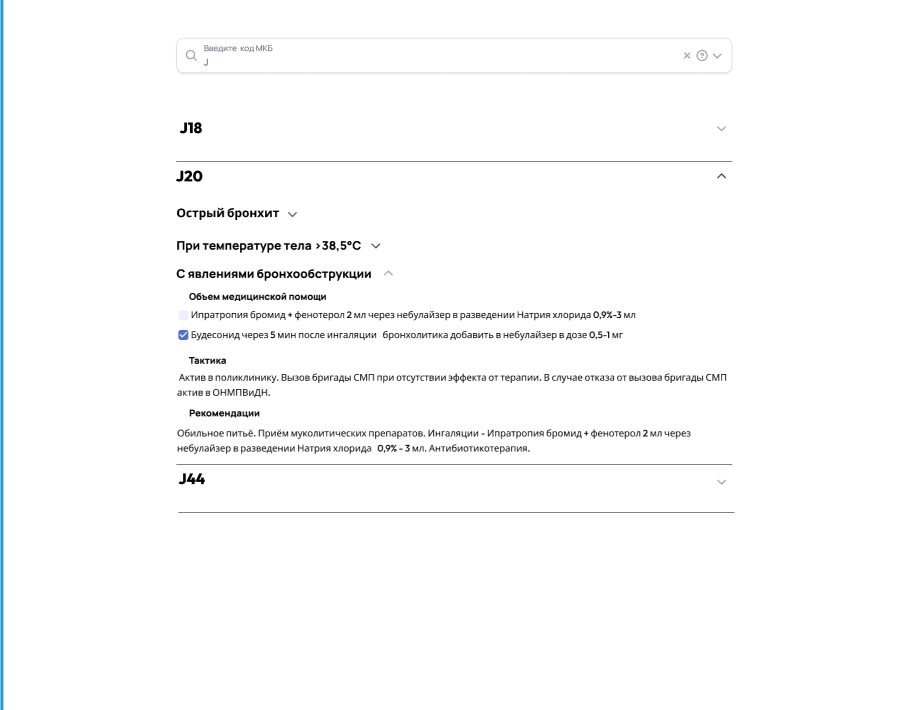
\includegraphics[scale=0.6]{styles/diploma/inc/prim.png}
        \caption{Интерфейс}
        \label{fig:fig12}
    \end{figure}
